

\section*{HS11. feladat:Gömb alakú főzőüst }
\addcontentsline{toc}{section}{HS/11. feladat}

\begin{tabular}{ | p{1.75cm} | p{11cm} | } 
	\hline
	Név: & Drávai Tamás László\\ 
	\hline
	Szak: & Mechatronikai mérnök \\ 
	\hline
	Félév: & 2019/2020 II. (tavaszi) félév \\ 
	\hline
\end{tabular}
\\
\\
HS11 feladat:\\
Egy 3 m (D1) külső átmérőjű gömb alakú víztartály 150mm vastag üvegpaplan szigeteléssel láttak el. Számítsuk ki a tartályba óránként beáramló hőmennyiséget valamint azt, hogy a tartályban lévő víz hőfoka óránként mennyit emelkedik.
\section*{Adatok}
$t_{sz}=50^{0}C $ A szigetelés külső felületének hőmérséklete
\\ 
$t_{b}=20^{0}C $ A tartály belső felületének hőmérséklete
\\ 
$\lambda_{sz}=0.037 \frac{W}{mK}\quad 
\rho_{víz} =998.2 \frac{W}{m^3} \quad 
c_{víz}=4.118 \frac{kJ}{kgK}$
\section*{Feladat megoldás}
$
\dot{Q} =\dfrac{4 \pi  \lambda_{sz}}{\dfrac{1}{r_2} - \dfrac{1}{r_1}} \cdot (T_b-T_{sz}) \\ 
\\\\
\dot{Q} =\dfrac{4 \pi  0.037 \dfrac{W}{mK } } {\dfrac{1}{1.65m} - \dfrac{1}{1.5m}}  \cdot (293.15K-323.15K)\\\\
\dot{Q}=-230.153 W=-230.153 \dfrac{J}{s}=-230.153 \dfrac{J}{s} \cdot 3600 =-828551.01\dfrac{J}{h}\\$
\begin{figure}[h]
	\centering
	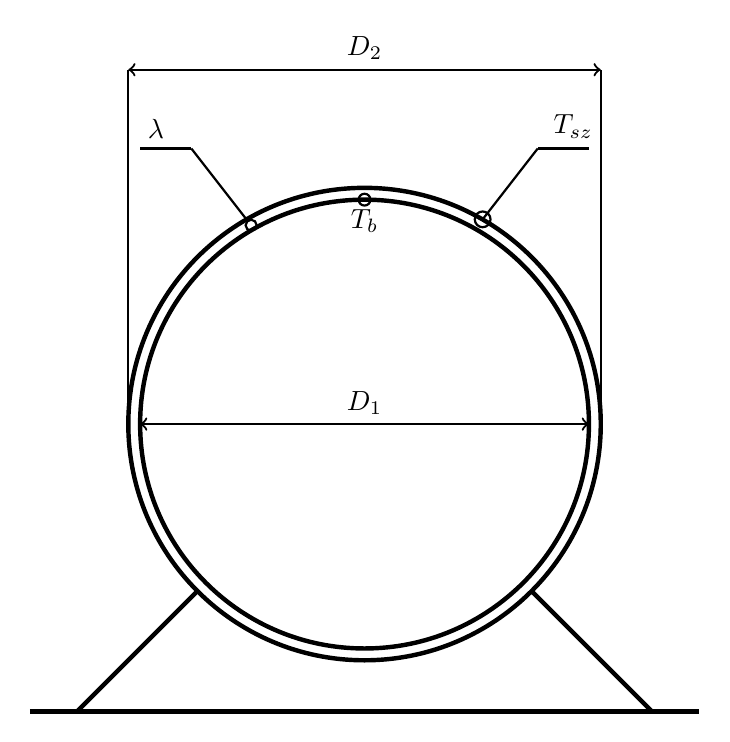
\begin{tikzpicture}
	%\draw[] (-6, -6) rectangle (6, 6);
	\draw[color =black, ultra thick] (0, 0) circle (30 mm); %külső fal	
	\draw[color =black,ultra thick] (0, 0) circle (2. 85) ;%belső fal 	
	\draw[thick,<->] (-2.85,0) -- (2.85,0);% méretnyíl
	\draw (0,0)  node[above] {$ D_1  $};
	\draw[thick,<->] (-3,4.5) -- (3,4.5); %felső méretnyíl
	\draw (0,4.5)  node[above] {$ D_2  $};
	\draw [thick] (-3,0) -- (-3,4.5) (3,0) -- (3,4.5); %%felső méretnyíl oldalt
	\draw [ultra thick] (-2.13,-2.13) -- (-3.65,-3.65) (2.13,-2.13) -- (3.65,-3.65); %lábak
	\draw [ultra thick] (-4.25,-3.65) -- (4.25,-3.65) ;%földvonal
	%Tsz
	\draw [thick] (1.5,2.6) circle (0.1) (1.5,2.6) -- (2.2,3.5)  ;
	\draw [thick]  (2.2,3.5) -- (2.85,3.5) ;
	\draw [thick](2.65,3.5)  node[above] {$T_{sz}$};
	% lambda
	\draw [thick] (-1.44,2.525) circle (0.07) (-1.5,2.6) -- (-2.2,3.5)  ;
	\draw [thick]  (-2.2,3.5) -- (-2.85,3.5) ;
	\draw [thick](-2.65,3.5)  node[above] {$\lambda$};
	%T2
	\draw [thick] (0,2.85) circle (0.075) ;
	\draw (0,2.85)  node[below] {$T_b$};	
	\end{tikzpicture}
	\caption{Gömb alakú főzőüst }
\end{figure}
\begin{figure}
	%\centering
	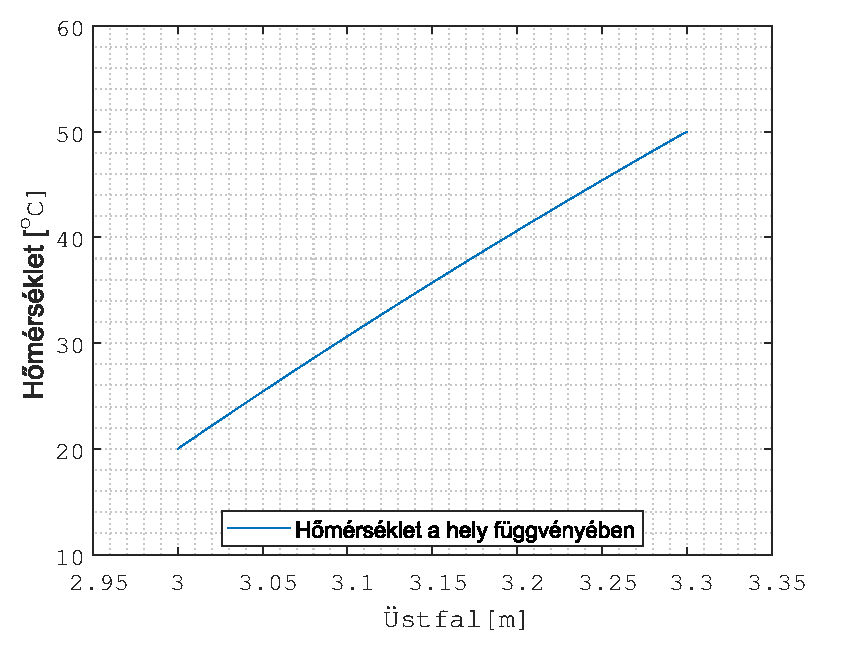
\includegraphics[width=1\linewidth]{homersekletfuggvenyHS11.eps}
	\caption{}
	\label{fig:waveforms}
\end{figure}
